\documentclass[12pt,twoside]{book}
\usepackage{layout}
%\usepackage{makeidx}
\RequirePackage{verbatim}
%\RequirePackage{alltt}
\usepackage{hyperref}
\usepackage{ifpdf}

\ifpdf 
   \pdfcompresslevel=9
   \pdfoutput=1
                                                                                            
                       
   \usepackage[pdftex]{graphicx}
   \usepackage[pdftex]{geometry}
   \usepackage[pdftex]{color}
   \usepackage{hyperref}
   \hypersetup{
     pdftitle={Recitation Activities for the Introduction to Differential Equations},
     pdfsubject={ODE},
     pdfauthor={Kelly Black},
     pdfkeywords={classroom activities},
     anchorcolor = {red},
     colorlinks = {true},
     %pdfpagemode={FullScreen}
   }
\else
   \usepackage{epsfig}
   \usepackage{color}
\fi



\pagestyle{myheadings}

%\setlength{\basicoddside}{\oddsidemargin}
%\setlength{\basicevenside}{\evensidemargin}
%\setlength{\basicwidth}{\textwidth}
%\setlength{\basictop}{\topmargin}
%\setlength{\basicheight}{\textheight}


\newcommand{\introduction}[1]{}

\font\tenit=cmti10
\makeatletter

\renewcommand{\@evenfoot}{\tenit Clarkson University Division of
  Mathematics and Computer Science \hfill}
\renewcommand{\@oddfoot}{\tenit \hfill Math 232: Introduction to
  Differential Equations - \today}

\renewcommand{\section}{\@startsection
  {section}
  {1}
  {0em}
  {\baselineskip}
  {-1em}
  {\normalfont\normalsize\bfseries}}

\renewcommand{\subsection}{\@startsection
  {subsection}
  {2}
  {0em}
  {\baselineskip}
  {-1em}
  {\normalfont\normalsize\bfseries}}

\renewcommand{\subsubsection}{\@startsection
  {subsubsection}
  {2}
  {0em}
  {\baselineskip}
  {-2em}
  {\normalfont\normalsize\itshape}}

\makeatother


\newlength{\basicoddside}
\newlength{\basicevenside}
\newlength{\basicwidth}
\newlength{\basictop}
\newlength{\basicheight}

\newcommand{\activityParams}{
  %\setlength{\hoffset}{0in}
  %\setlength{\oddsidemargin}{-0.5in}
  %\setlength{\evensidemargin}{-0.5in}
  %\setlength{\textwidth}{7.5in}
  \setlength{\topmargin}{-0.5in}
  \setlength{\textheight}{9in}
}

\newcommand{\textParams}{
  \setlength{\oddsidemargin}{\basicoddside}
  \setlength{\evensidemargin}{\basicevenside}
  \setlength{\textwidth}{\basicwidth}
  \setlength{\topmargin}{\basictop}
  \setlength{\textheight}{\basicheight}
}


  \setlength{\oddsidemargin}{-0.25in}
  \setlength{\evensidemargin}{0.25in}
  \setlength{\textwidth}{6.25in}
  \setlength{\topmargin}{-0.5in}
  \setlength{\textheight}{9in}
  \setlength{\marginparwidth}{56pt}


\newcommand{\sideNote}[1]{\marginpar{\tenit \raggedright #1}}
\newcommand{\doNotPrint}[1]{}


\newtheorem{lemma}{Lemma}[subsection]
\newtheorem{theorem}{Theorem}[subsection]



\newcounter{activity}
\setcounter{activity}{1}

\newcommand{\actTitle}[1]{
  \cleardoublepage
  \activityParams
  \stepcounter{activity}
  \markboth
  {Name: \hspace*{2.5in} \hfil  Activity: \theactivity}
  {Name: \hspace*{2.5in} \hfil  Activity: \theactivity}
  \stepcounter{subsection}
  \addcontentsline{toc}{subsection}{
    \protect\numberline{\thesubsection}{#1}}
}

\newcounter{hw}
\setcounter{hw}{0}
\newcommand{\hwTitle}[1]{
  \cleardoublepage
  \activityParams
  \stepcounter{hw}
  \markboth
  {Name: \hspace*{2.5in} \hfil  Home Work: \thehw}
  {Name: \hspace*{2.5in} \hfil  Home Work: \thehw}
  \stepcounter{subsubsection}
  \addcontentsline{toc}{subsubsection}{
    \protect\numberline{\thesubsubsection}{#1}}
}

\newcommand{\preClass}[1]{
  \cleardoublepage
  \activityParams
  \markboth
  {Name: \hspace*{2in} \hfil Preclass Work - Finish Before Class Begins \hfil}
  {Name: \hspace*{2in} \hfil Preclass Work - Finish Before Class Begins \hfil}
  \stepcounter{subsubsection}
  \addcontentsline{toc}{subsubsection}{
    \protect\numberline{\thesubsubsection}{#1}}
}

\newcommand{\postClass}{

  \cleardoublepage
  \activityParams
  \markboth
  {Name: \hspace*{2in} \hfil Postclass Work - Finish After Class \hfil}
  {Name: \hspace*{2in} \hfil Postclass Work - Finish After Class \hfil}
%  \stepcounter{subsubsection}
%  \addcontentsline{toc}{subsubsection}{
%    \protect\numberline{\thesubsubsection}{#1}}
}


\newcounter{quiz}
\setcounter{quiz}{1}
\newcommand{\qzTitle}[1]{
  \cleardoublepage
  \activityParams
  \stepcounter{quiz}
  \markboth
  {Name: \hspace*{2.5in} \hfil  #1 Quiz: \thequiz}
  {Name: \hspace*{2.5in} \hfil  #1 Quiz: \thequiz}
  \stepcounter{subsubsection}
  \addcontentsline{toc}{subsubsection}{
    \protect\numberline{\thesubsubsection}{#1}}
}


\newcommand{\stateSummary}{\item State and summarize two ideas from today's
  class. 
  \vfill 
  \centerline{\textit{(Over)}}
  \clearpage }


\newcommand{\addTOC}[1]{
  \stepcounter{section}
  \addcontentsline{toc}{section}{
    \protect\numberline{\thesection}{#1}}
  }



\newenvironment{problem}
{\begin{list}
{\arabic{enumi}.}
{\usecounter{enumi}
\setlength{\rightmargin}{0pt}
%\setlength{\rightmargin}{-72pt}
\setlength{\parsep}{1em}
\setlength{\listparindent}{0pt}
}}
{\end{list}}

\newenvironment{subproblem}
{\begin{list}
{(\alph{enumii})}
{\usecounter{enumii}
\setlength{\rightmargin}{0pt}
\setlength{\parsep}{1em}
\setlength{\listparindent}{0pt}
}}
{\end{list}}

\newenvironment{multiEqn}
{\begin{eqnarray*} 
 \begin{array}{rclclclcl}}
{\end{array}
 \end{eqnarray*}}


\setcounter{activity}{0}


\newcommand{\arrayTwo}[4]{
  \left[
  \begin{array}{rr}
    #1 & #2 \\
    #3 & #4
  \end{array}
  \right]
}


\newcommand{\vecTwo}[2]{
  \left[
  \begin{array}{r}
    #1 \\  #2
  \end{array}
  \right]
}

\newcommand{\stateTwo}[2]{
  \begin{array}{rr}
    \mbox{\fontsize{6}{6}\selectfont $#1$} \\  \mbox{\fontsize{6}{6}\selectfont $#2$}
  \end{array}
}


\newcommand{\startRowOpsTwo}{
  \left[
    \begin{array}{rr|rr}
}

\newcommand{\oneRowOpsTwo}[4] {
      #1 & #2 & #3 & #4 \\
}


\newcommand{\startRowOpsThree}{
  \left[
    \begin{array}{rrr|rrr}
}


\newcommand{\stopRowOps}{
    \end{array}
  \right]
}


\newcommand{\vecFour}[4]{
  \left[
  \begin{array}{r}
    #1 \\  #2 \\ #3 \\ #4
  \end{array}
  \right]
}




\begin{document}


\title{Recitation Activities for the Introduction to Differential
  Equations}
\author{Kelly Black\\Clarkson University\\Division of Mathematics and
  Computer ScienceR}

\maketitle



\begin{center}
  
  
\includegraphics{ccV3}

  Recitation Activities for the Introduction to Differential Equations
  by Kelly Black is licensed under a Creative Commons
  Attribution-NonCommercial-ShareAlike 3.0 Unported License.

  \url{http://creativecommons.org/licenses/by-nc-sa/3.0/ }

\end{center}


\clearpage


\actTitle{Basic Integrals and Slope Fields}
\begin{problem}
\item Find the solutions to the following integrals. In each case
  solve for $y$ in terms of $t$. (Do not forget the ``$+C$'' for each
  integral!)
  \begin{subproblem}
    \item $y = \int \cos(3t) ~ dt$
      \vfill
    \item $y = \int t^2 + e^{5t} ~ dt$
      \vfill
    \item $t = \int \frac{1}{y} ~ dy$
      \vfill
    \item $t = \int y^2 ~ dy$
      \vfill
  \end{subproblem}

\clearpage

\item For each slope field make sketches for different solutions for
  each of the following initial conditions:
  \begin{eqnarray*}
    y(0) & = & 3, \\
    y(0) & = & 1, \\
    y(0) & = & 0, \\
    y(0) & = & -1, \\
    y(0) & = & -3.
  \end{eqnarray*}
  For each slope field state the general behavior and state the long
  term solutions if they exist.

  \begin{subproblem}
    \item 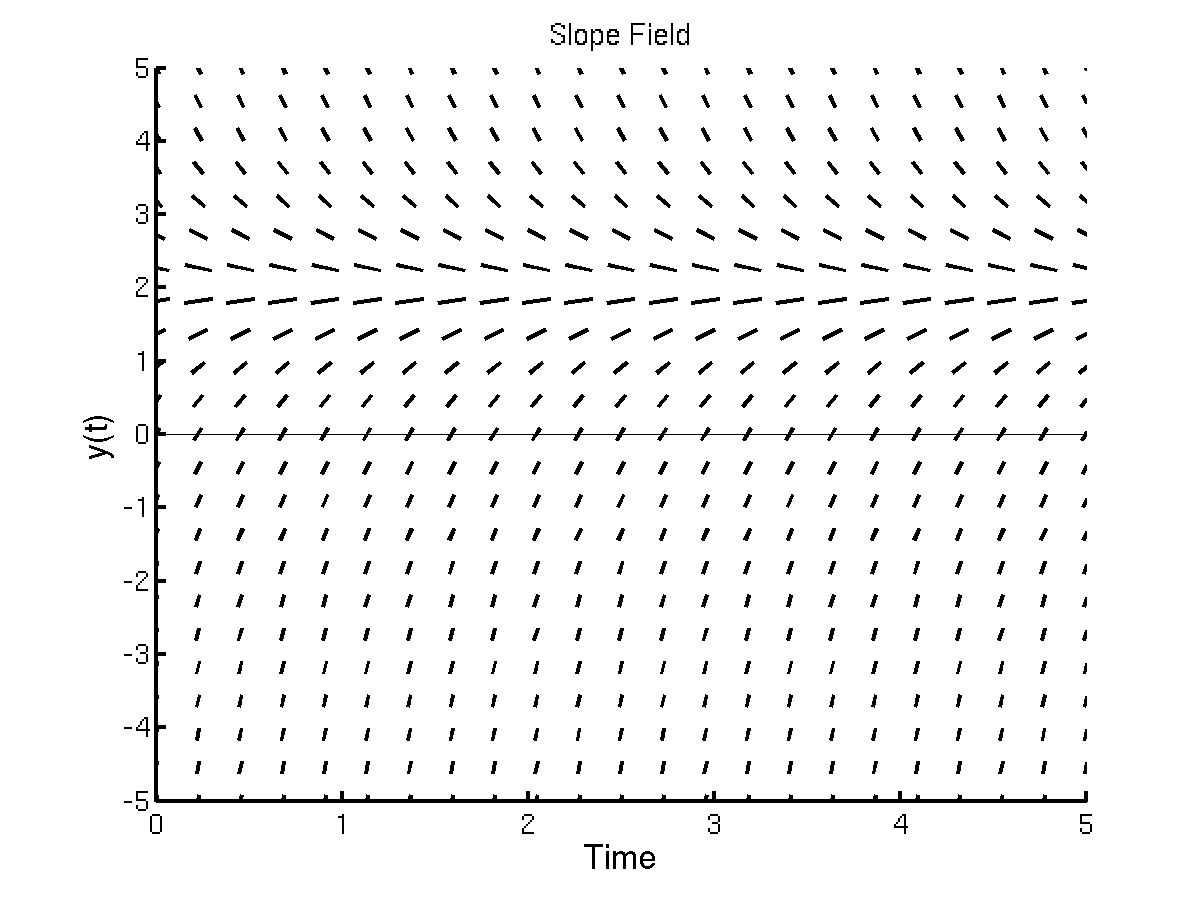
\includegraphics[height=3.0in]{sfSteadyWk1}
    \item 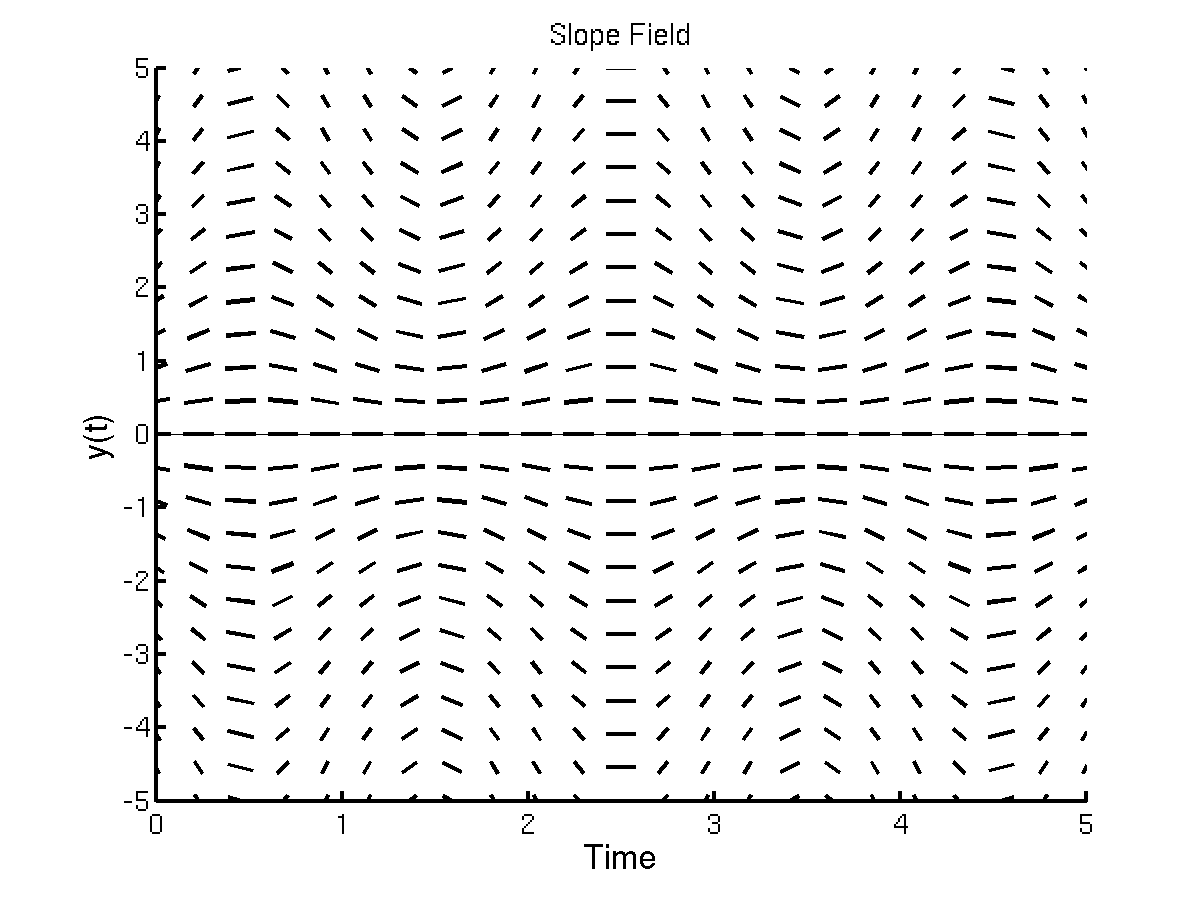
\includegraphics[height=3.0in]{sfOscillateWk1}

      \clearpage

    \item 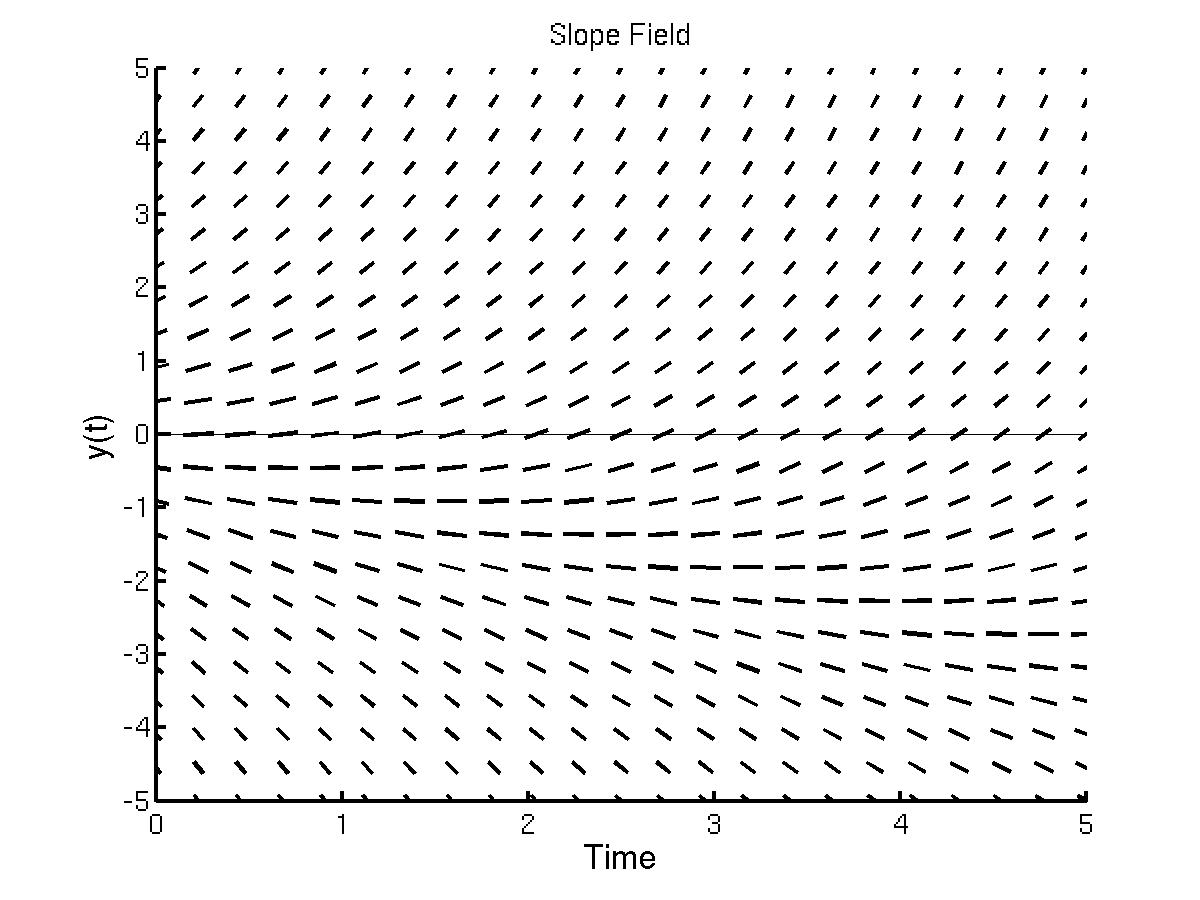
\includegraphics[height=4.0in]{sfLinearWk1}
    \item 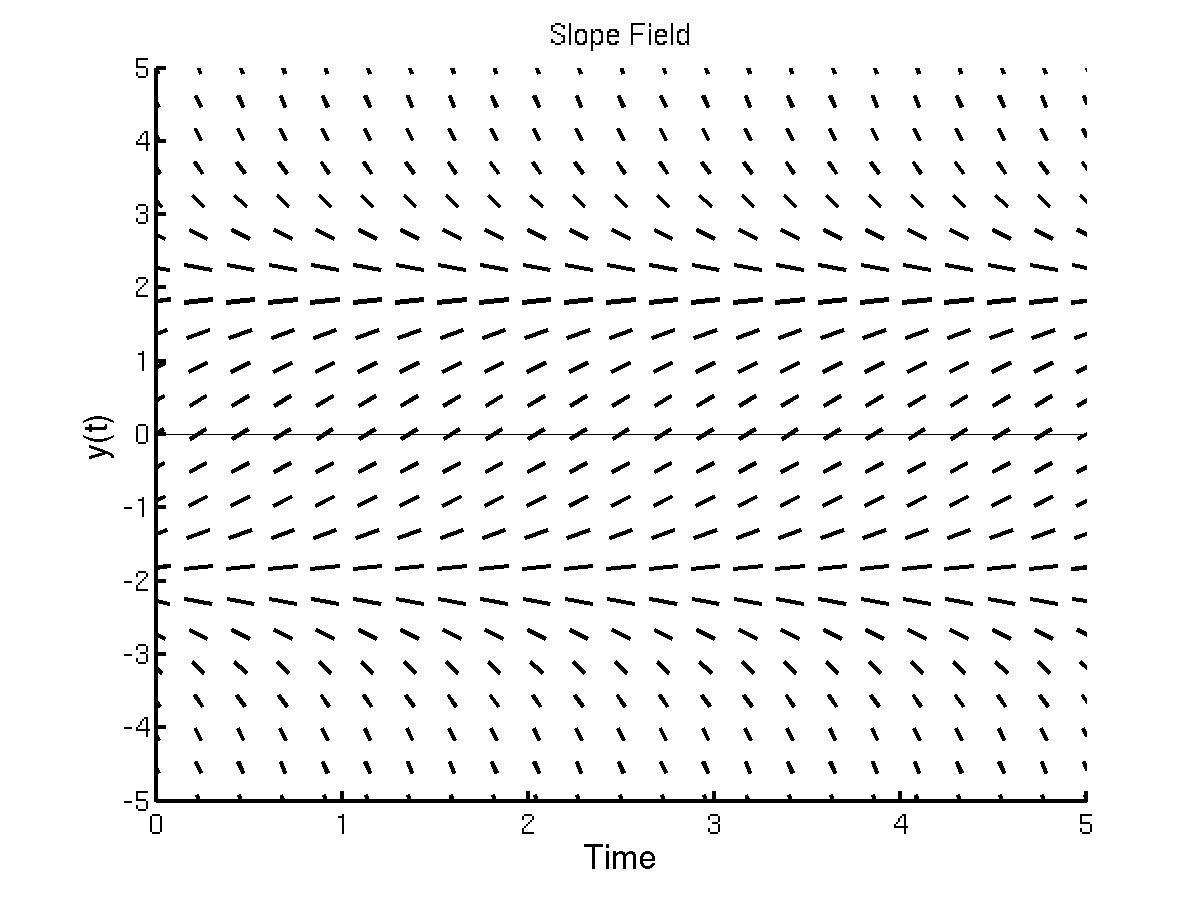
\includegraphics[height=4.0in]{sfStabilityWk1}

  \end{subproblem}

\end{problem}


\actTitle{The Chain Rule}
\begin{problem}
  \item Suppose that $3t+C=\ln(y(t))$ where $C$ is a constant. Solve
    the equation for $y(t)$.

    \vfill

  \item The function $y(t)$ depends on $t$. Use the chain rule to find
    the derivative of $\ln(y(t))$.
    \vfill

    \clearpage

  \item Show that the relationship $3t+C=\ln(y(t))$ can also be
    expressed as $y'=3y$.

    \vfill

  \item Show that for any constant $k$ the function
    \begin{eqnarray*}
      y(t) & = & k e^{5t}
    \end{eqnarray*}
    is a solution to the differential equation 
    \begin{eqnarray*}
      y' & = & 5y.
    \end{eqnarray*}
    \vfill

\end{problem}

  \actTitle{Separable ODEs}
  \begin{problem}
  \item Expand each expression using partial fractions:
    \begin{subproblem}
    \item $\frac{y}{y^2-4}$
      \vfill

    \item $\frac{4}{y^2-2y}$.
      \vfill
      
    \item $\frac{3}{y^2-3y+2}$
      \vfill

    \end{subproblem}
    \clearpage
  \item Find the solutions to the following ODEs. 
    \begin{subproblem}
    \item $y' = y^2 + 1$, $y(0)=3$.
      \vfill
    \item $y' = yt - t$, $y(0)=4$.
      \vfill
    \item $y'=y(y-1)$, $y(0)=5$.
      \vfill
    \item $y' = y^2(y+1)$, $y(0)=10$.
      \vfill
    \end{subproblem}

  \end{problem}


  \actTitle{Linear Differential Equations}
  For each problem below $C_1$ and $C_2$ are constants.
  \begin{problem}

  \item Show that $y=C_1 e^{3t}-\frac{1}{3}$ is a solution to the
    differential equation $y'=3y+1$.
    \vfill

  \item Show that $y=C_1 e^{t} + C_2 e^{-2t}$ is a solution to the
    differential equation $y''+3y'+2y=0$.

    \vfill

    \clearpage

  \item Suppose that you have the following differential equation:
    \begin{eqnarray*}
      \frac{d}{dt} \left( y(t) e^{3t} \right) & = & e^{3t}.
    \end{eqnarray*}
    Take the antiderivative of each side and express the result
    without any derivatives. (Do not forget the constant of
    integration.)  
    
    \vfill

  \item Simplify the expression and solve for $y(t)$. 
    \vfill

    \clearpage

  \item Suppose that $y$ is a function of $t$. Use the product rule to
    find the derivative of the function $\left(y(t) e^{3t}\right)$.
    \vfill

  \item Suppose that the expression in the previous problem is equal
    to $e^{3t}$.  Set the previous expression equal to $e^{3t}$ and
    simplify. What is the new differential equation?
    \vfill

  \item What is the solution to the differential equation?

\end{problem}


  \actTitle{Growth and Decay}
  \begin{problem}
  \item Find the solution to the following differential equation:
    \begin{eqnarray*}
      A' & = & -0.1 A, \\
      A(0) & = & 1,000.
    \end{eqnarray*}
    What is the long term solution?
    \vfill
    \clearpage
  \item The number of bacteria in a colony at 10:00am is approximately
    five million. At noon the number is approximately seven
    million. How many bacteria were in the colony at 9:00am?
    \vfill
  \end{problem}


  \actTitle{Mixing}
  \begin{problem}

  \item A tank initially contains 2,000 litres of water with a
    concentration of mercury of $6.0\times 10^{-5}$ grams per
    litre. Water that contains $3.0\times 10^{-5}$ grams per litre is
    pumped into the tank at 100 litres per hour. The well mixed
    solution is pumped out of the tank at 100 litres per hour.  How
    long will it take for the concentration in the tank to reach
    $4.5\times 10^{-5}$ grams per litre?

    \begin{subproblem}
      \item Draw a picture. Label and define the important quantities.
        \vfill

      \item Define the quantity to use. Determine the rate that
        mercury moves into the tank, and determine the rate that
        mercury moves out of the tank. Define the initial condition.
        \vfill

        \clearpage

      \item Write out the differential equation and solve it to find
        the amount of mercury in the tank at any time. Once you find a
        formula for the amount of mercury determine the formula for
        the concentration at any time.

        \vfill
        

    \end{subproblem}



\end{problem}


\preClass{Linear Theory}

\begin{problem}
\item Expand each of the expressions below. (You will need to ``FOIL''
  the expressions.) In each case treat the parameter $i$ as a
  constant.

  \begin{subproblem}
  \item $(4+3i)*(5-6i)$
    \vfill

  \item $(2+i)(10+4i)$
    \vfill
      
  \item $(2-i)(2+i)$
    \vfill

  \item $(6+3i)(6-3i)$
    \vfill

  \end{subproblem}
\end{problem}



  \actTitle{Complex Numbers}
  \begin{problem}
  \item Find the solution to the following differential equation:
    \begin{eqnarray*}
      y' & = & k y, \\
      y(0) & = & 1.
    \end{eqnarray*}
    \vfill

  \item Replace the constant ``k'' with a constant called ``$i$'' and
    find the solution to the following differential equation:
    \begin{eqnarray*}
      y' & = & i y, \\
      y(0) & = & 1.
    \end{eqnarray*}
    \vfill


    \clearpage
  \item Define the constant ``i'' to be $\sqrt{-1}$. Find each of the
    following values:

    \begin{subproblem}
      \item $i^2$
        \vfill
      \item $i^3$
        \vfill
      \item $i*(1+i)$
        \vfill
    \end{subproblem}

  \end{problem}


  \actTitle{Complex Numbers}
  \begin{problem}

  \item Define $y(t)$ to be the following function:
    \begin{eqnarray*}
      y(t) & = & \cos(t) + i \sin(t).
    \end{eqnarray*}
    Answer each of the following questions. Keep in mind that $i$ is a
    constant.

    \begin{subproblem}
      \item Determine the derivative of $y(t)$. 
        \vfill

      \item Determine and simplify $i*y(t)$.
        \vfill

        \clearpage

      \item Show that $y(t)$ is a solution to the following
        differential equation:
        \begin{eqnarray*}
          y' & = & i y, \\
          y(0) & = & 1.
        \end{eqnarray*}

        \vfill

      \item Recall the solution of the previous differential equation
        given on the first page of these activities. (Write it down here.)
        \vfill

      \item What is the relationship between that solution and the
        function $y(t)$?
        \vfill
        

    \end{subproblem}

    \clearpage

  \item Express the variable $x$ in terms of $r$ and $\theta$. Do the
    same for $y$. Determine how to find $r$ and $\theta$ given $x$ and
    $y$. 

    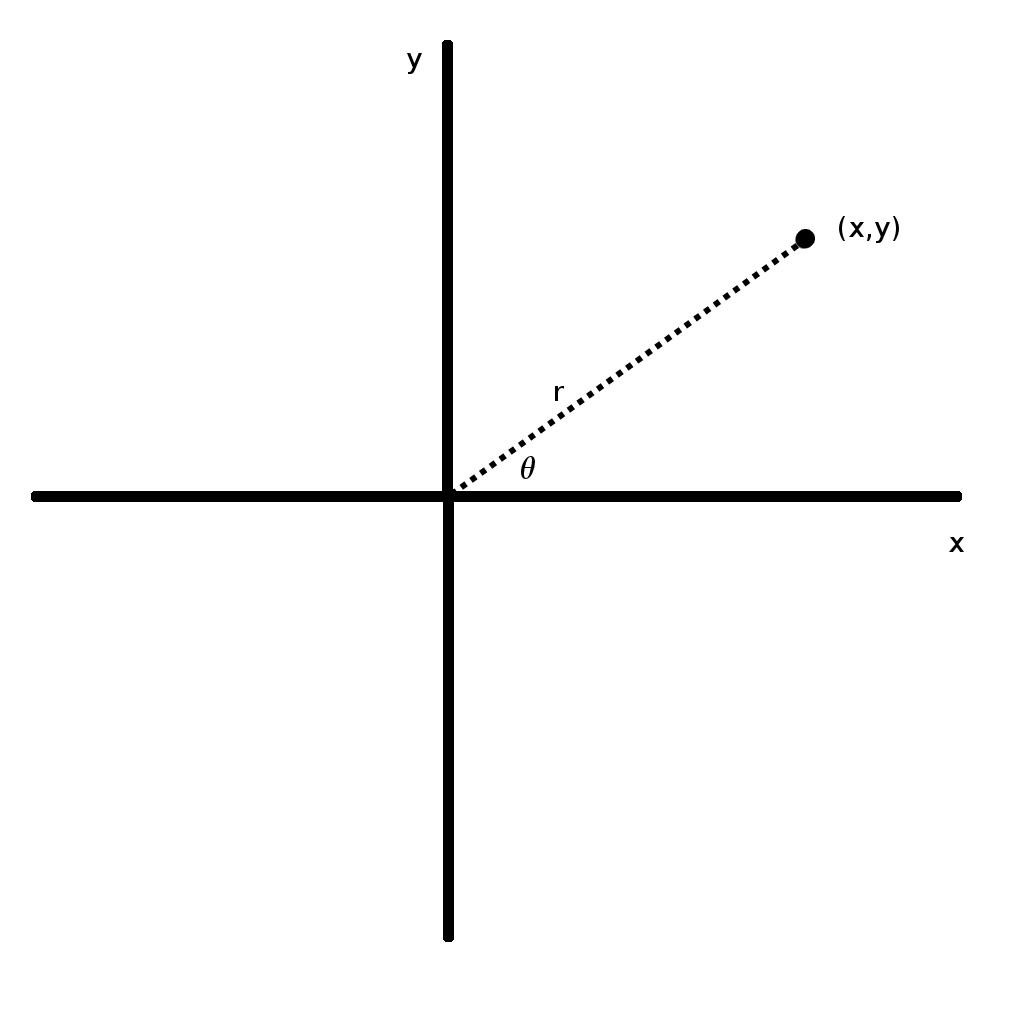
\includegraphics[height=12cm]{polar}
    \vfill


  \end{problem}


\preClass{Complex Numbers}

\begin{problem}
\item Plot and then convert each point in the complex plane into polar
  coordinates. Label the radius and angle in each case.

  \begin{subproblem}
  \item $3+7i$
    \vfill

  \item $-3+7i$
    \vfill
      
  \item $-4+2i$
    \vfill

  \item $3-1i$
    \vfill

  \end{subproblem}
\end{problem}


  \actTitle{Complex Numbers}
  \begin{problem}
  \item Expand and simplify the following expressions:
    \begin{subproblem}
      \item $(1+i)(3-i)$
        \vfill

      \item $(3+2i)(1-i)(7+2i)$
        \vfill

      \item $\frac{1+2i}{4+7i}$
        \vfill

      \item $\frac{\bar{4-i}}{3-i}(2+i)$
        \vfill

    \end{subproblem}

    \clearpage

  \item Express each of the following numbers in the form $a+bi$:
    \begin{subproblem}
    \item $e^{i\pi/4}$
      \vfill
    \item $2e^{i 3\pi/2}$
      \vfill
    \item $10e^{i \pi/3}$
      \vfill
    \item $4e^{i \pi}$
      \vfill
    \end{subproblem}


  \end{problem}


  \actTitle{Complex Numbers}
  \begin{problem}

  \item Plot each of the following numbers in the complex plane and
    then express them in Euler form:
    \begin{subproblem}
      \item $1+i$
        \vfill
      \item $i-i$
        \vfill
      \item $-1+2i$
        \vfill
      \item $-3-i$
        \vfill
    \end{subproblem}

    \clearpage

  \item Determine the values of the roots. For each problem show the
    graphical representation of the root in relation to the number
    that you are taking the root of.
    \begin{subproblem}
      \item $\sqrt[4]{i}$. 
        \vfill

      \item $\sqrt[3]{1}$.
        \vfill

      \item $\sqrt{-4}$.
        \vfill

      \item $\sqrt[5]{1+i}$.
        \vfill

    \end{subproblem}

    \clearpage



  \end{problem}

  \actTitle{Linear Algebra}
  \begin{problem}
  \item 
    \vfill

  \item 
    \vfill


    \clearpage
  \item 

    \begin{subproblem}
      \item 
        \vfill
      \item 
        \vfill
      \item 
        \vfill
    \end{subproblem}

  \end{problem}


  \actTitle{Linear Algebra}
  \begin{problem}

  \item 

    \begin{subproblem}
      \item 
        \vfill

      \item 
        \vfill

        \clearpage

      \item 

        \vfill

      \item 
        \vfill

      \item 
        \vfill
        

    \end{subproblem}

    \clearpage

  \item 
    \vfill


\end{problem}



  \actTitle{Inverse of a matrix}
  \begin{problem}
  \item Given the following matrix
    \begin{eqnarray*}
      A & = & \arrayTwo{1}{2}{1}{-4}
    \end{eqnarray*}
    \begin{subproblem}
      \item Does the inverse exist? (Determine the answer without
        finding the inverse.)
        \vfill
      \item Is there a unique solution to the equation
        \begin{eqnarray*}
          A \vec{x} & = & \vec{b}
        \end{eqnarray*}
        for any vector $\vec{b}$?
        \vfill
      \item Are the columns of the matrix linearly independent?
        \vfill
    \end{subproblem}

    \clearpage
  \item Find the inverse of the matrix.

        \vfill
        
  \end{problem}


  \actTitle{Linear Dependence}
  \begin{problem}

    \item Determine whether or not the set of functions whose first
      derivative is zero at $x=0$ is a vector space.
      \vfill

    \item Determine whether or not the set of functions that are equal
      to one at $x=0$ is a vector space.
      \vfill

      \clearpage

  \item Are the following vectors linearly independent? If so find a
    way to express one of the vectors in terms of the others

    \begin{eqnarray*}
      \vecFour{1}{2}{-1}{-2},~\vecFour{3}{6}{-3}{-6},~\vecFour{-4}{-10}{5}{11},
      ~\vecFour{2}{7}{-3}{-9}
    \end{eqnarray*}


\end{problem}

  \actTitle{Second Order Equations}
  \begin{problem}
  \item The following questions refer to the following differential
    equation:
    \begin{eqnarray*}
      y'' - y - 12 = 0.
    \end{eqnarray*}

    \begin{subproblem}
      \item Show that $y=e^{4t}$ is a solution.
        \vspace{4cm}
      \item Show that $y=e^{-3t}$ is a solution.
        \vspace{4cm}
      \item Show that $y=C_1 e^{4t} + C_2 e^{-3t}$ is a solution for
        any constants $C_1$ and $C_2$. Will the solution grow or
        decay?

        \vfill

    \end{subproblem}
 
    \clearpage
  \item Find the solutions to the following differential equation:
    \begin{eqnarray*}
      y'' + 3y' - 10y = 0.
    \end{eqnarray*}
    Determine if the solution will exhibit growth or decay. Can you
    determine the answer to the question of stability by only looking
    at the roots of the characteristic equation? If so how?

    \vfill
  \end{problem}


  \actTitle{Second Order Equations}
  \begin{problem}

  \item The questions refer to the following differential equation:
    \begin{eqnarray*}
      y'' + 4y & = & 0.
    \end{eqnarray*}

    \begin{subproblem}
      \item Show that $y=C_1 e^{i2t} + C_2 e^{-i2t}$ is a solution to
        the differential equation.
        \vfill

      \item Use Euler's formula to write the solution, $y=C_1 e^{i2t}
        + C_2 e^{-i2t}$, in terms of sines and cosines.
        \vfill

        \clearpage

      \item Simplify the terms so that the sine and cosine terms are
        only expressed by either $\sin(2t)$ or $\cos(2t)$.

        \vfill

      \item Collect all the sine terms and the cosine terms so that
        the solution is in the form
        \begin{eqnarray*}
          y & = & \#_1 \cos(2t) + \#_2 \sin(2t).
        \end{eqnarray*}
        \vfill

      \item Show that $y=k_1 \cos(2t) + k_2 \sin(2t)$ is a solution to
        the original differential equation.
        \vfill
        

    \end{subproblem}


\end{problem}



\preClass{Second order, constant coefficient equations.}

  \begin{problem}

  \item A spring mass system is constructed. The mass is 0.1 kg. The
    spring is stretched 0.04 m when the mass is hung vertically from
    the spring. The force due to air friction is estimated to be 0.03
    N when the object is moving at 0.2 m/sec. The system is placed in
    a horizontal orientation, and the object is pulled so that the
    spring extends 0.03 m and released from rest.

    \begin{subproblem}
      \item Determine the governing equation for the system. (This
        includes the initial conditions.)
        \vfill

      \item Determine the \textit{general} solution to the differential
        equation. (Do not consider the initial conditions yet.)
        \vfill

        \clearpage

      \item Determine the specific solution to match the initial conditions.

        \vfill

      \item Determine a different value for the spring constant so
        that the system will oscillate with a period of 1.2 seconds.
        \vfill

    \end{subproblem}



  \end{problem}


\actTitle{Second order, linear differential equations}

\begin{problem}
\item A spring mass system is constructed. The mass is $m$ kg. The
  spring is stretched 0.04 m when the mass is hung vertically from the
  spring. The air friction coefficient is $b$.

    \begin{subproblem}
      \item Determine the governing equation for the system. 
        \vfill

      \item Determine the characteristic equation for the differential
        equation. (Do not consider the initial conditions yet.)
        \vfill

        \clearpage

      \item Assume that the solution to the characteristic equation
        will be a complex number so that the system will
        oscillate. Break the solutions into two pieces, the real and
        the imaginary parts.

        \vfill

      \item Find and solve the system of equations that result for $m$
        and $b$ if you wish the amplitude of the system to decay like
        $e^{-t/10}$ and the system to oscillate with a period of 3.1
        seconds.

        \vfill

    \end{subproblem}


\end{problem}


\actTitle{Method of Undetermined Coefficients}

  \begin{problem}
  \item Find the solution to the following differential equation:
    \begin{eqnarray*}
      y'' - 2y' - 8y & = & 3t + 4.
    \end{eqnarray*}
    \begin{subproblem}
    \item Write out the homogeneous equation.
      \vspace{2em}
    \item Find the solution to the homogeneous equation.
      \vfill

    \clearpage

  \item Write out the general form of the particular solution:
    \vspace{2em}

  \item Substitute your particular solution into the non-homogeneous equation.
    \vfill

  \item Solve for the constants.
    \vfill

  \end{subproblem}

  \end{problem}



\preClass{Linear Algebra}

\begin{problem}
\item 

  \begin{subproblem}
  \item A system of equations is given by
    \begin{eqnarray*}
      \left[
        \begin{array}{rr}
          12 & -1 \\
          4 & 7
        \end{array}
      \right] \vec{x} & = & \vec{b}.
    \end{eqnarray*}
    Is the solution to the system unique?
    \vfill

  \item A system of equations is given by
    \begin{eqnarray*}
      \left[
        \begin{array}{rr}
          4 & 6 \\
          2 & 3
        \end{array}
      \right] \vec{x} & = & \vec{b}.
    \end{eqnarray*}
    Is the solution to the system unique?
    \vfill
      
  \end{subproblem}
\end{problem}

  \actTitle{Linear Algebra}
  \begin{problem}
  \item Find all possible values of $\lambda$ so that the following system of
    equations 
    \begin{eqnarray*}
      \left[ \begin{array}{rr}
          1-\lambda & 8 \\
          2 & 1-\lambda
        \end{array} \right]
      \vec{v} & = & \vec{0}
    \end{eqnarray*}
    does \textbf{not} have a unique solution.

    \vfill

  \item Define the matrix A to be
    \begin{eqnarray*}
      \left[ \begin{array}{rr}
          1 & 8 \\
          2 & 1
        \end{array} \right].
    \end{eqnarray*}
    Show that the system of equations given by
    \begin{eqnarray*}
      A \vec{v} & = & \lambda \vec{v}
    \end{eqnarray*}
    reduces to the same system given in the problem above. Note: the
    constant $\lambda$ is a scalar, and you cannot subtract a matrix
    from a scalar so you will have to use the identity matrix.

    \vfill


    \clearpage
  \item Using the same system given in the first problem let
    $\lambda=-3$ and $\vec{v}=\left[\begin{array}{r} x_1 \\
        x_2 \end{array} \right]$.  Put the equations into an augmented
    matrix and solve for $x_1$ and $x_2$. Write the solution as a
    linear combination of some vector.

    \vfill

  \end{problem}


  \actTitle{Linear Algebra}
  \begin{problem}

  \item Repeat the steps that you used on the previous activity for
    the matrices given below.
    
    \begin{subproblem}
      
    \item Find values of $\lambda$ and vectors $\vec{v}$ that satisfy
      $A\vec{v}=\lambda\vec{v}$ where 
        \begin{eqnarray*}
          A &  = & 
          \left[ \begin{array}{rr}
               8 &  6 \\
              -9 & -7
            \end{array} \right].
        \end{eqnarray*}

        \vfill
        \clearpage


      \item Find values of $\lambda$ and vectors $\vec{v}$ that satisfy
        $A\vec{v}=\lambda\vec{v}$ where 
        \begin{eqnarray*}
          A & = & 
          \left[ \begin{array}{rr}
              10 &  -6 \\
              18 & -11
            \end{array} \right].
        \end{eqnarray*}

        \vfill
        \clearpage

    \end{subproblem}


\end{problem}



\preClass{Linear Algebra}

\begin{problem}
\item 

  \begin{subproblem}
  \item Find the eigen values and eigen vectors for the following matrices:
    \begin{eqnarray*}
      \left[
        \begin{array}{rr}
          12 & -1 \\
          4 & 7
        \end{array}
      \right].
    \end{eqnarray*}
    \vfill

  \item A system of equations is given by
    \begin{eqnarray*}
      \left[
        \begin{array}{rr}
          4 & 6 \\
          2 & 3
        \end{array}
      \right].
    \end{eqnarray*}
    \vfill
      
  \end{subproblem}
\end{problem}

\actTitle{Linear Algebra}
\begin{problem}
\item Express the following second order differential equation as a
  system of two equations:
  \begin{eqnarray*}
    x'' - 3x & = & 0, \\
    x(0) & = & 1.0, \\
    x'(0) & = & 0.0
  \end{eqnarray*}
  Find the eigen vectors and eigen values for the system. Compare the
  eigen values to the roots of the characteristic equation of the
  original equation. Compare the solution to the system to the
  solution to the original equation.

  \vfill



  \clearpage

\item Express the following second order differential equation as a
  system of two equations:
  \begin{eqnarray*}
    x'' - 2x' - 3x & = & 0, \\
    x(0) & = & -2.0, \\
    x'(0) & = & 1.0
  \end{eqnarray*}
    Find the eigen vectors and eigen values for the system. Compare
    the eigen values to the roots of the characteristic equation of
    the original equation. Compare the solution to the system to the
    solution to the original equation.

    \vfill


  \end{problem}


  \actTitle{Linear Algebra}
  \begin{problem}

  \item Two tanks are arranged so that they exchange their
    contents. The first tank initially contains 300 liters of fresh
    water. Water that contains 5 g/liter of a chemical is pumped in at
    a rate of 4 liters/minute. The well mixed solution is pumped into
    the second tank at a rate of 6 liters per minute.

    The second tank initially contains 200 liters of fresh water. The
    well mixed solution is pumped into the first tank at a rate of 6
    liters per minute. Additionally, the solution is pumped out at a
    rate of 4 liters/minute.


    \begin{subproblem}
      \item Draw a picture. Then determine and organize the given
        information. Define and label the variables that represent the
        amount of chemical in each tank.
        \vfill

      \item Determine the differential equation for the first tank.
        \vfill

      \item Determine the differential equation for the second tank.
        \vfill

      \item Write the equations as a system of differential equations.
        \vfill

    \end{subproblem}

    \clearpage

  \item For each of the following systems of differential equations
    sketch the solution trajectories in the phase plane for each
    equation.
    
    \begin{subproblem}
      
    \item 
        \begin{eqnarray*}
          \frac{d}{dt} \vec{x} & = & 
          \left[ \begin{array}{rr}
               8 &  6 \\
              -9 & -7
            \end{array} \right] \vec{x}.
        \end{eqnarray*}

        \vfill
        \clearpage


      \item 
        \begin{eqnarray*}
          \frac{d}{dt} \vec{x} & = & 
          \left[ \begin{array}{rr}
              10 &  -6 \\
              18 & -11
            \end{array} \right] \vec{x}.
        \end{eqnarray*}

        \vfill
        \clearpage

    \item 
        \begin{eqnarray*}
          \frac{d}{dt} \vec{x} & = & 
          \left[ \begin{array}{rr}
               -6 & -6 \\
                1 & -1
            \end{array} \right] \vec{x}.
        \end{eqnarray*}

        \vfill
        \clearpage


      \item 
        \begin{eqnarray*}
          \frac{d}{dt} \vec{x} & = & 
          \left[ \begin{array}{rr}
              -5 &  -12 \\
               4 &    9
            \end{array} \right] \vec{x}.
        \end{eqnarray*}

        \vfill


    \end{subproblem}


\end{problem}




\end{document}
